% Created 2019-04-05 vie 12:41
% Intended LaTeX compiler: pdflatex
\documentclass[11pt]{article}
\usepackage[utf8]{inputenc}
\usepackage[T1]{fontenc}
\usepackage{graphicx}
\usepackage{grffile}
\usepackage{longtable}
\usepackage{wrapfig}
\usepackage{rotating}
\usepackage[normalem]{ulem}
\usepackage{amsmath}
\usepackage{textcomp}
\usepackage{amssymb}
\usepackage{capt-of}
\usepackage{hyperref}
\author{Karen Guadalupe Lechuga Trejo}
\date{\today}
\title{Programación lineal}
\hypersetup{
 pdfauthor={Karen Guadalupe Lechuga Trejo},
 pdftitle={Programación lineal},
 pdfkeywords={},
 pdfsubject={},
 pdfcreator={Emacs 25.2.2 (Org mode 9.2.3)}, 
 pdflang={English}}
\begin{document}

\maketitle
\tableofcontents


\section{Teoría}
\label{sec:org589280a}
\subsection{Motivación}
\label{sec:org68ab1d9}

El objetivo de la programación lineal es es maximizar funciones
lineales sobre dominios convexos, es decir, definidos sobre regiones
dadas por desigualdades.

\begin{center}
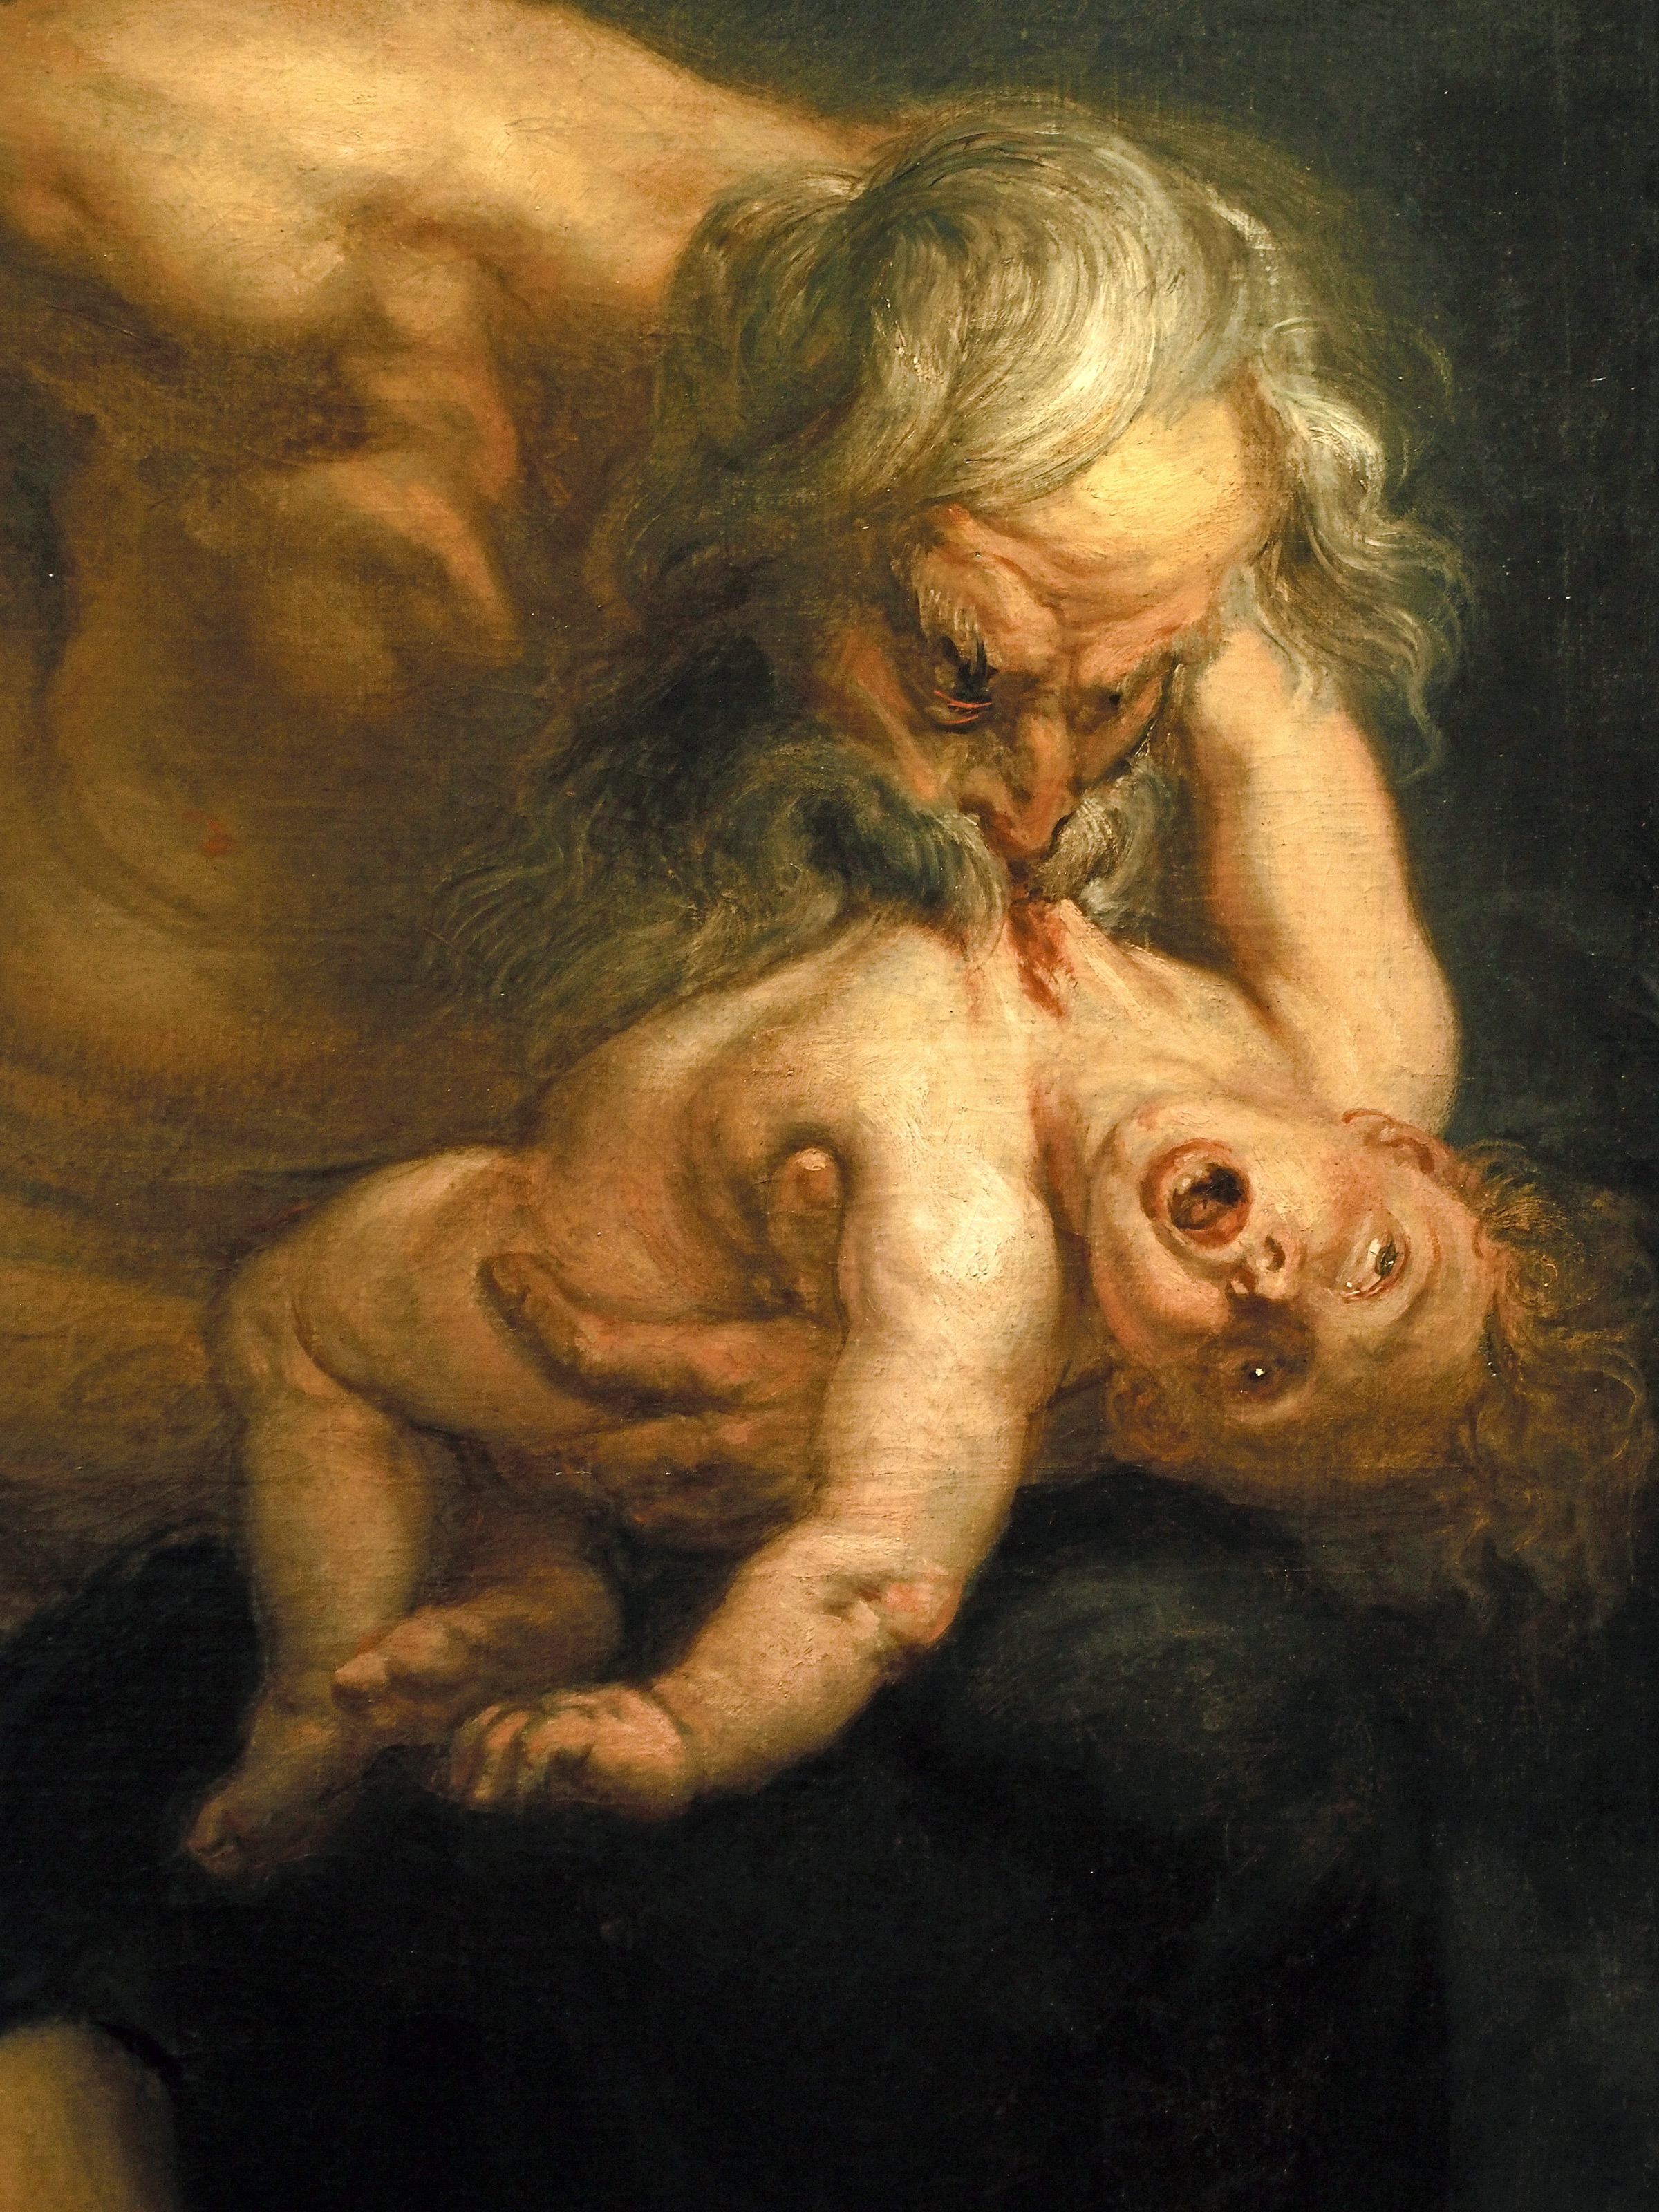
\includegraphics[width=.9\linewidth]{Rubens-Saturno-detalle.jpg}
\end{center}

\subsection{Ejemplos}
\label{sec:org0ba3090}

\begin{itemize}
\item El problema de la dieta.
\item Optimización de lugares en una excursión.
\item Escoger objetos óptimos para un campamento.
\item El problema del flujo máximo.
\end{itemize}

\subsection{Convexidad}
\label{sec:orga16a443}

Un conjunto \(X\) es \textbf{convexo} si para todos \(x,y\in X\) y
\(t\in[0,1]\) se tiene que \(tx + (1-t)y \in X\).
\subsection{Método SIMPLEX}
\label{sec:orgde8861b}

\section{Herramientas computacionales}
\label{sec:orgb85ae47}
\subsection{Emacs}
\label{sec:org5e6f372}

\begin{center}
\begin{tabular}{ll}
C-x C-s & salvar archivo\\
C-x C-f & abrir archivo\\
M-q & formatear párrafo\\
C-x d & editar directorios\\
C-g & interrumpe procesos\\
C-x 1 & regresa a una sola pantalla\\
C-x 2 & divide horizontalmente\\
C-x 3 & divide verticalmente\\
M-w & copiar la región\\
C-w & borrar la región\\
shift-flechas & seleccionar la región\\
C-y & pegar la región\\
C-c C-e & menú exportar en otros formatos\\
M-flechas & mover renglones/columnas de tabla\\
\end{tabular}
\end{center}


\subsection{Git}
\label{sec:org600acc4}
\begin{enumerate}
\item Github
\label{sec:orga3b6696}
\end{enumerate}
\subsection{Python}
\label{sec:orgfe3c51b}
\begin{enumerate}
\item Lenguaje Python
\label{sec:orga36f304}
\item Jupyter
\label{sec:org8f1ebd1}
\end{enumerate}
\subsection{\LaTeX{}}
\label{sec:org2fa556f}
\end{document}